\maketitle

\newpage

\section{Proposta}

O presente estudo tem como objetivo desenvolver uma metodologia capaz de comparar, selecionar, combinar e aprimorar técnicas de processamento de imagem para a detecção e classificação de falhas em isoladores. Para isso, serão estabelecidas métricas para avaliar a eficácia dos processamentos de imagem, considerando aspectos como acurácia e tempo de processamento. Além disso, serão construídos modelos de redes neurais para avaliar o desempenho dos processamentos, podendo abranger tarefas como classificação, detecção e regressão. No decorrer do estudo, serão construídos modelos de redes neurais voltados para a avaliação do desempenho das técnicas de processamento de imagem, sem a intenção de definir um modelo ideal.

Também será analisado o impacto da escolha do modelo de rede neural no desempenho do processamento, visto que diferentes modelos podem gerar distintos resultados para um mesmo processamento. A influência do dataset na eficácia do processamento será outro aspecto a ser investigado, considerando possíveis variações nos resultados devido ao uso de diferentes conjuntos de dados. Para aprimorar os processamentos de imagem, será desenvolvida uma metodologia que permita a combinação de diferentes processamentos unitários (processamentos de imagem que realizam uma única operação). Além disso, será criado um método de ajuste automático de parâmetros das técnicas de processamento de imagem, com o intuito de otimizar seus resultados sem exigir extensa intervenção manual.

A metodologia proposta será desenvolvida dentro de um conjunto de restrições previamente estabelecidas, garantindo um escopo bem delimitado e viável dentro do período de realização da dissertação. Primeiramente, o estudo será restrito à detecção e classificação de falhas em isoladores elétricos, não abrangendo outros componentes elétricos. O uso de imagens previamente adquiridas será uma diretriz, de modo que apenas imagens já disponíveis ou capturadas por métodos convencionais serão utilizadas, sem o desenvolvimento de novas técnicas de aquisição de imagens. Além disso, a metodologia será aplicada exclusivamente a técnicas de processamento de imagem já conhecidas, sem a criação de novos algoritmos de base.

Os modelos de redes neurais desenvolvidos terão o propósito único de avaliar o impacto das redes sobre os processamentos de imagem, sem a intenção de definir um modelo definitivo para diagnóstico industrial. A análise será conduzida utilizando conjuntos de dados já existentes ou obtidos por métodos convencionais, sem a necessidade de criar um novo dataset específico para o estudo. A otimização contemplada estará limitada ao ajuste de parâmetros das técnicas existentes, não incluindo o desenvolvimento de novas abordagens baseadas em inteligência artificial para otimização dos processamentos. Por fim, toda a avaliação será realizada em ambiente controlado, sem a realização de testes em ambientes industriais reais.

A Figura \ref{fig:proposta} ilustra o diagrama da proposta de metodologia.

\begin{figure}[h]
    \centering
    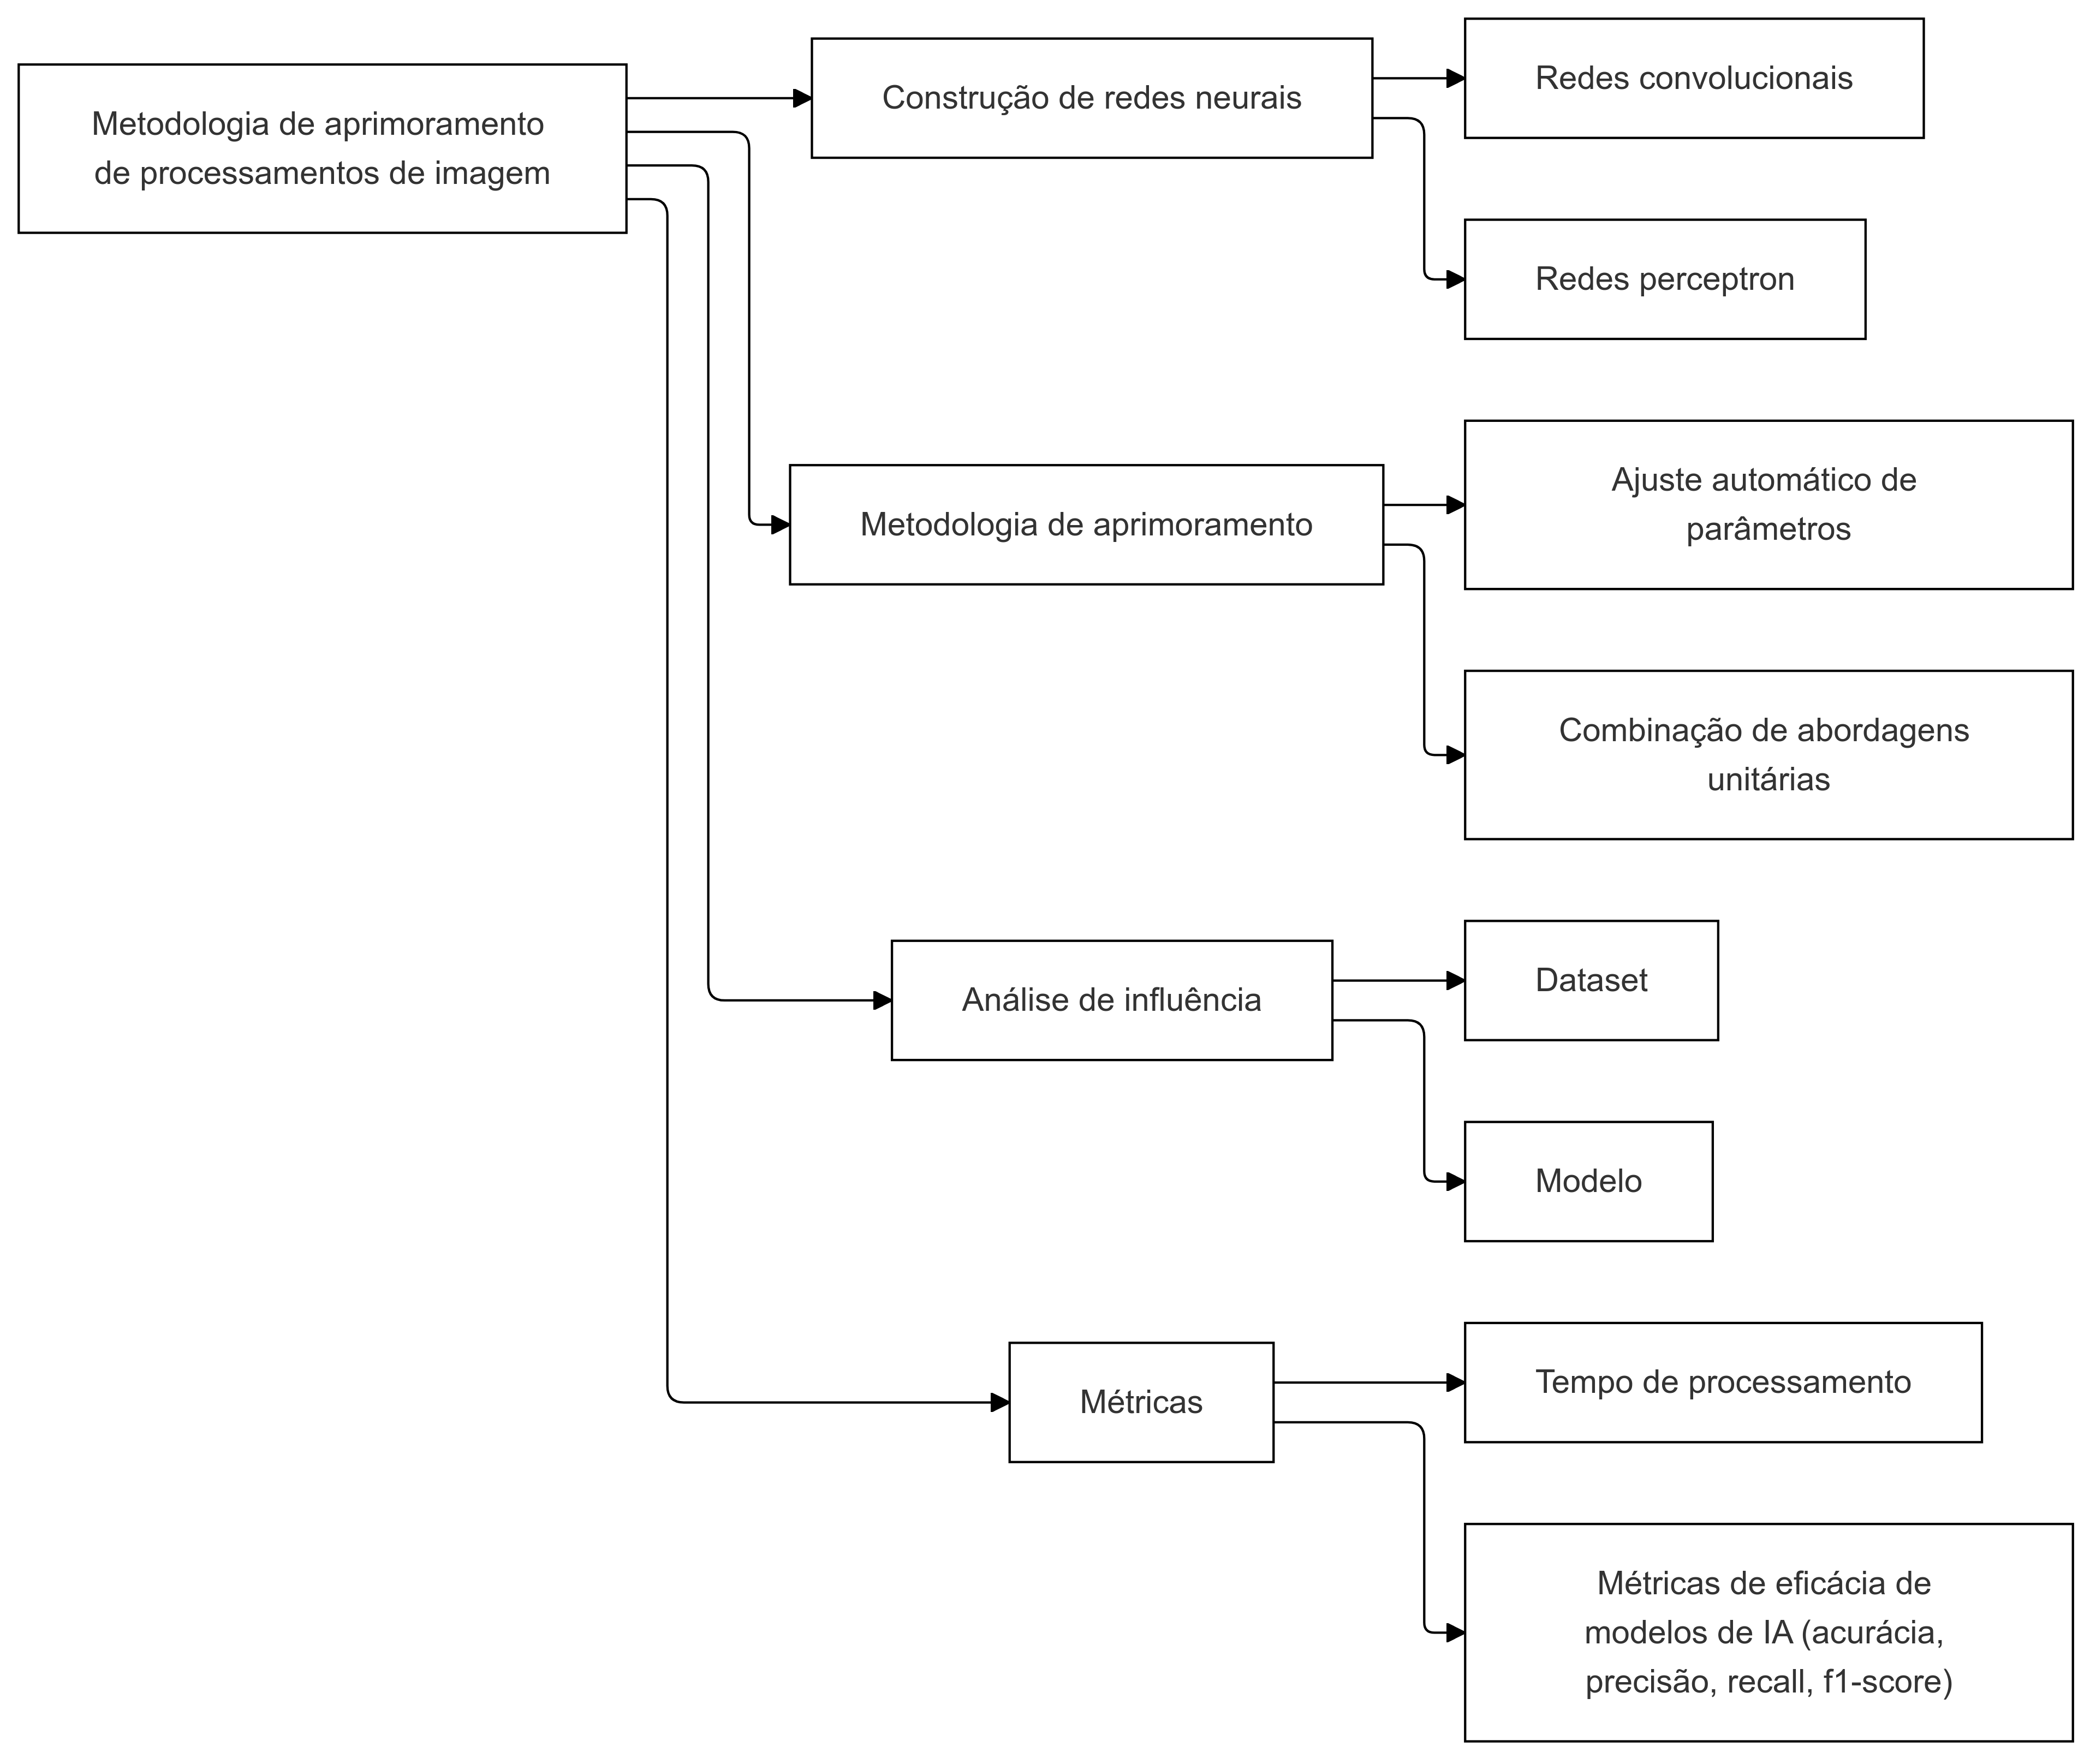
\includegraphics[width=\textwidth]{img/proposta.png}
    \caption{Diagrama da proposta de metodologia}
    \label{fig:proposta}
\end{figure}

\subsection{Objetivo geral}

O objetivo geral deste estudo é desenvolver uma metodologia capaz de comparar, selecionar, combinar e aprimorar técnicas de processamento de imagem para a detecção e classificação de falhas em isoladores.

\subsection{Objetivos específicos}

Para alcançar esse objetivo, foram definidos os seguintes objetivos específicos:

\begin{itemize}
    \item Estabelecer métricas para avaliar a eficácia dos processamentos de imagem, considerando aspectos como acurácia e tempo de processamento.
    \item Determinar o tipo de modelo de redes neurais ideal para avaliar o desempenho dos processamentos, podendo abranger classificação, detecção e regressão.
    \item Construir modelos de redes neurais destinados à avaliação do desempenho das técnicas de processamento de imagem, sem o intuito de encontrar um modelo definitivo.
    \item Analisar o impacto da escolha do modelo de rede neural no desempenho do processamento, considerando que diferentes modelos podem gerar diferentes resultados para um mesmo processamento.
    \item Avaliar a influência do dataset na eficácia do processamento, considerando possíveis variações nos resultados devido à utilização de diferentes conjuntos de dados.
    \item Desenvolver uma metodologia para o aprimoramento dos processamentos de imagem por meio da combinação de diferentes abordagens unitárias.
    \item Criar um método de ajuste automático de parâmetros dos processamentos de imagem, visando otimizar seus resultados sem a necessidade de intervenção manual extensa.
\end{itemize}